%-*-latex-*-
\sectionthree{Merge}
\begin{python0}
from solutions import *; clear()
\end{python0}

Suppose you're two max heaps.
Is there an efficient way to put them together to get a max heap?
This is called a heap \defone{merge} or a heap \defone{union}.

For instance suppose, suppose a machine has
two exact same server process running the same software,
answering to HTTP requests.
Each server software maintains it's own queue of server requests.
However something bad happened: one of the server process is stuck
(hackers?)
A main master process that watches the two server processes
sees that one of server processes is stuck.
So it transfers the queue of requests to the one that is still alive
and kills the server that is stuck.
Somehow the two queues of requests has to be merged.

By the way.
I hope you realize that if you have a max heap and you remove the
root, then the two subtrees are themselves max heaps.
For instance if you remove the root from this max heap:


\begin{center}

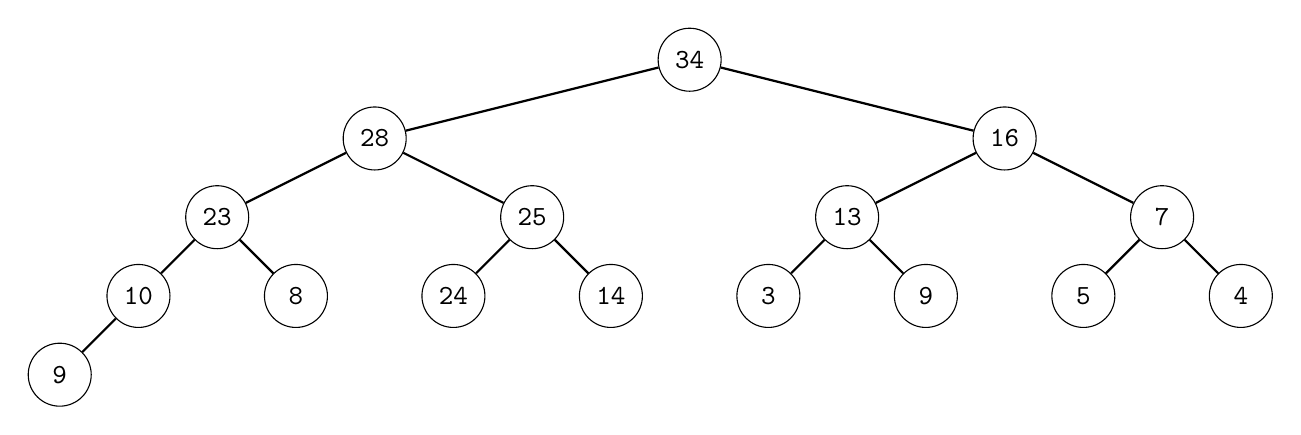
\begin{tikzpicture}
\node at (8,-1) [circle,draw,minimum size=8mm] (A) {\texttt{34}};
\node at (4,-2) [circle,draw,minimum size=8mm] (B) {\texttt{28}};
\node at (12,-2) [circle,draw,minimum size=8mm] (C) {\texttt{16}};
\node at (2,-3) [circle,draw,minimum size=8mm] (D) {\texttt{23}};
\node at (6,-3) [circle,draw,minimum size=8mm] (E) {\texttt{25}};
\node at (10,-3) [circle,draw,minimum size=8mm] (F) {\texttt{13}};
\node at (14,-3) [circle,draw,minimum size=8mm] (G) {\texttt{7}};
\node at (1,-4) [circle,draw,minimum size=8mm] (H) {\texttt{10}};
\node at (3,-4) [circle,draw,minimum size=8mm] (I) {\texttt{8}};
\node at (5,-4) [circle,draw,minimum size=8mm] (J) {\texttt{24}};
\node at (7,-4) [circle,draw,minimum size=8mm] (K) {\texttt{14}};
\node at (9,-4) [circle,draw,minimum size=8mm] (L) {\texttt{3}};
\node at (11,-4) [circle,draw,minimum size=8mm] (M) {\texttt{9}};
\node at (13,-4) [circle,draw,minimum size=8mm] (N) {\texttt{5}};
\node at (15,-4) [circle,draw,minimum size=8mm] (O) {\texttt{4}};
\node at (0,-5) [circle,draw,minimum size=8mm] (P) {\texttt{9}};
\draw [-,thick] (A) -- (B);
\draw [-,thick] (A) -- (C);
\draw [-,thick] (B) -- (D);
\draw [-,thick] (B) -- (E);
\draw [-,thick] (C) -- (G);
\draw [-,thick] (C) -- (F);
\draw [-,thick] (D) -- (H);
\draw [-,thick] (D) -- (I);
\draw [-,thick] (E) -- (J);
\draw [-,thick] (E) -- (K);
\draw [-,thick] (F) -- (L);
\draw [-,thick] (F) -- (M);
\draw [-,thick] (G) -- (N);
\draw [-,thick] (G) -- (O);
\draw [-,thick] (H) -- (P);

;
\end{tikzpicture}
    
\end{center}



you get the left subtree which is a max heap:

\begin{center}
\begin{tikzpicture}

\fill[white] (0.0, 0.0) circle (0.3);
\node [line width=0.03cm,black,minimum size=0.57cm,draw,circle] at (0.0,0.0)(5){};\draw (0.0, 0.0) node[color=black] {\texttt{5}};
\fill[white] (-1.5, -1.0) circle (0.3);
\node [line width=0.03cm,black,minimum size=0.57cm,draw,circle] at (-1.5,-1.0)(2){};\draw (-1.5, -1.0) node[color=black] {\texttt{2}};
\fill[white] (1.5, -1.0) circle (0.3);
\node [line width=0.03cm,black,minimum size=0.57cm,draw,circle] at (1.5,-1.0)(10){};\draw (1.5, -1.0) node[color=black] {\texttt{10}};
\fill[white] (-2.25, -2.0) circle (0.3);
\node [line width=0.03cm,black,minimum size=0.57cm,draw,circle] at (-2.25,-2.0)(0){};\draw (-2.25, -2.0) node[color=black] {\texttt{0}};
\fill[white] (-0.75, -2.0) circle (0.3);
\node [line width=0.03cm,black,minimum size=0.57cm,draw,circle] at (-0.75,-2.0)(3){};\draw (-0.75, -2.0) node[color=black] {\texttt{3}};
\fill[white] (2.25, -2.0) circle (0.3);
\node [line width=0.03cm,black,minimum size=0.57cm,draw,circle] at (2.25,-2.0)(18){};\draw (2.25, -2.0) node[color=black] {\texttt{18}};\draw[line width=0.03cm,black,->,>=triangle 60] (5) to  (2);
\draw[line width=0.03cm,black,->,>=triangle 60] (5) to  (10);
\draw[line width=0.03cm,black,->,>=triangle 60] (10) to  (18);
\draw[line width=0.03cm,black,->,>=triangle 60] (2) to  (0);
\draw[line width=0.03cm,black,->,>=triangle 60] (2) to  (3);
\end{tikzpicture}

\end{center}



and the right subtree which is also a max heap:


\begin{center}

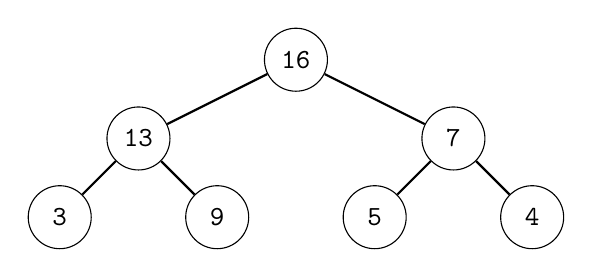
\begin{tikzpicture}
\node at (3,-1) [circle,draw,minimum size=8mm] (C) {\texttt{16}};
\node at (1,-2) [circle,draw,minimum size=8mm] (F) {\texttt{13}};
\node at (5,-2) [circle,draw,minimum size=8mm] (G) {\texttt{7}};
\node at (0,-3) [circle,draw,minimum size=8mm] (L) {\texttt{3}};
\node at (2,-3) [circle,draw,minimum size=8mm] (M) {\texttt{9}};
\node at (4,-3) [circle,draw,minimum size=8mm] (N) {\texttt{5}};
\node at (6,-3) [circle,draw,minimum size=8mm] (O) {\texttt{4}};
\draw [-,thick] (C) -- (G);
\draw [-,thick] (C) -- (F);
\draw [-,thick] (F) -- (L);
\draw [-,thick] (F) -- (M);
\draw [-,thick] (G) -- (N);
\draw [-,thick] (G) -- (O);

;
\end{tikzpicture}
    
\end{center}



OK.
Back to the algorithm of merging two (max) heaps $H_0$ and $H_1$.
Suppose the total number of nodes in $H_1$ is $m$
and the total number of nodes in $H_2$ is $n$.
Without using the existing heap structure in $H_1$ and $H_2$
and just build a heap from scratch requires $O(n)$ using the build-heap
operation.
Also, note that if we can merge two heaps quickly,
then another way to build a heap is to do it recursively:
recursive divide a collection of values into two piles,
make them into heaps, then merge the heaps.
So what's there not to like?

However, for our max heap, the only way seems to be to copy the
values from one heap to another and perform build-heap
which will run in $O(m + n)$
where $m$ is the size of the first heap and $n$ is the size of the second.


%-*-latex-*-

\begin{ex} 
  \label{ex:prob-00}
  \tinysidebar{\debug{exercises/{disc-prob-28/question.tex}}}

  \solutionlink{sol:prob-00}
  \qed
\end{ex} 
\begin{python0}
from solutions import *
add(label="ex:prob-00",
    srcfilename='exercises/discrete-probability/prob-00/answer.tex') 
\end{python0}


\begin{comment}
\begin{center}
\begin{tikzpicture}

\fill[white] (0.0, 0.0) circle (0.3);
\node [line width=0.03cm,black,minimum size=0.57cm,draw,circle] at (0.0,0.0)(5){};\draw (0.0, 0.0) node[color=black] {\texttt{5}};
\fill[white] (-3.0, -1.0) circle (0.3);
\node [line width=0.03cm,black,minimum size=0.57cm,draw,circle] at (-3.0,-1.0)(2){};\draw (-3.0, -1.0) node[color=black] {\texttt{2}};
\fill[white] (3.0, -1.0) circle (0.3);
\node [line width=0.03cm,black,minimum size=0.57cm,draw,circle] at (3.0,-1.0)(10){};\draw (3.0, -1.0) node[color=black] {\texttt{10}};
\fill[white] (-4.5, -2.0) circle (0.3);
\node [line width=0.03cm,black,minimum size=0.57cm,draw,circle] at (-4.5,-2.0)(0){};\draw (-4.5, -2.0) node[color=black] {\texttt{0}};
\fill[white] (-1.5, -2.0) circle (0.3);
\node [line width=0.03cm,black,minimum size=0.57cm,draw,circle] at (-1.5,-2.0)(3){};\draw (-1.5, -2.0) node[color=black] {\texttt{3}};
\fill[white] (4.5, -2.0) circle (0.3);
\node [line width=0.03cm,black,minimum size=0.57cm,draw,circle] at (4.5,-2.0)(15){};\draw (4.5, -2.0) node[color=black] {\texttt{15}};
\fill[white] (5.25, -3.0) circle (0.3);
\node [line width=0.03cm,black,minimum size=0.57cm,draw,circle] at (5.25,-3.0)(18){};\draw (5.25, -3.0) node[color=black] {\texttt{18}};\draw[line width=0.03cm,black,->,>=triangle 60] (5) to  (2);
\draw[line width=0.03cm,black,->,>=triangle 60] (5) to  (10);
\draw[line width=0.03cm,black,->,>=triangle 60] (10) to  (15);
\draw[line width=0.03cm,black,->,>=triangle 60] (2) to  (0);
\draw[line width=0.03cm,black,->,>=triangle 60] (2) to  (3);
\draw[line width=0.03cm,black,->,>=triangle 60] (15) to  (18);
\end{tikzpicture}

\end{center}


[Instead of max heap, what is the levels are
coordinates?
I.e., the max is root,
the 2nd and 3rd at level 1,
the 4th,5th,6th,7th at level 2, etc.
If so, then during merge, to new heap's root is one of the two roots.
Say the first heap has a large root.
Then heap1's level 0 is done.
For level 1 of teh new heap, we look at level 1 of heap1
and level0 of heap2.
Etc.

\begin{center}
\begin{tikzpicture}

\fill[white] (0.0, 0.0) circle (0.3);
\node [line width=0.03cm,black,minimum size=0.57cm,draw,circle] at (0.0,0.0)(5){};\draw (0.0, 0.0) node[color=black] {\texttt{5}};
\fill[white] (-3.0, -1.0) circle (0.3);
\node [line width=0.03cm,black,minimum size=0.57cm,draw,circle] at (-3.0,-1.0)(2){};\draw (-3.0, -1.0) node[color=black] {\texttt{2}};
\fill[white] (3.0, -1.0) circle (0.3);
\node [line width=0.03cm,black,minimum size=0.57cm,draw,circle] at (3.0,-1.0)(15){};\draw (3.0, -1.0) node[color=black] {\texttt{15}};
\fill[white] (-4.5, -2.0) circle (0.3);
\node [line width=0.03cm,black,minimum size=0.57cm,draw,circle] at (-4.5,-2.0)(0){};\draw (-4.5, -2.0) node[color=black] {\texttt{0}};
\fill[white] (-1.5, -2.0) circle (0.3);
\node [line width=0.03cm,black,minimum size=0.57cm,draw,circle] at (-1.5,-2.0)(3){};\draw (-1.5, -2.0) node[color=black] {\texttt{3}};
\fill[white] (1.5, -2.0) circle (0.3);
\node [line width=0.03cm,black,minimum size=0.57cm,draw,circle] at (1.5,-2.0)(10){};\draw (1.5, -2.0) node[color=black] {\texttt{10}};
\fill[white] (4.5, -2.0) circle (0.3);
\node [line width=0.03cm,black,minimum size=0.57cm,draw,circle] at (4.5,-2.0)(18){};\draw (4.5, -2.0) node[color=black] {\texttt{18}};\draw[line width=0.03cm,black,->,>=triangle 60] (5) to  (2);
\draw[line width=0.03cm,black,->,>=triangle 60] (5) to  (15);
\draw[line width=0.03cm,black,->,>=triangle 60] (15) to  (10);
\draw[line width=0.03cm,black,->,>=triangle 60] (15) to  (18);
\draw[line width=0.03cm,black,->,>=triangle 60] (2) to  (0);
\draw[line width=0.03cm,black,->,>=triangle 60] (2) to  (3);
\end{tikzpicture}

\end{center}



In the above, 16 should probably be moved the the subtree at 28.
Who can replaced 16?
The max of 16's children is 13.
Or just looking at the subtree at 16, maybe it's better to switch 7 and 9:

\begin{center}
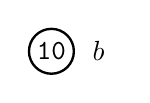
\begin{tikzpicture}

\fill[white] (0.0, 0.0) circle (0.3);
\node [line width=0.03cm,black,minimum size=0.57cm,draw,circle] at (0.0,0.0)(10){};\draw (0.0, 0.0) node[color=black] {\texttt{10}};
\fill[white] (0.6, 0.0) circle (0.3);
\node [draw=none,line width=0cm,black,minimum size=0.6cm,circle] at (0.6,0.0){};\draw (0.6, 0.0) node[color=black] {$b$};
\end{tikzpicture}

\end{center}



or

\begin{center}
\begin{tikzpicture}


\node at (8,-1) [circle,draw,minimum size=8mm] (A) {\texttt{34}};
\node at (4,-2) [circle,draw,minimum size=8mm] (B) {\texttt{28}};
\node at (12,-2) [circle,draw,minimum size=8mm] (C) {\texttt{16}};
\node at (2,-3) [circle,draw,minimum size=8mm] (D) {\texttt{23}};
\node at (6,-3) [circle,draw,minimum size=8mm] (E) {\texttt{25}};
\node at (10,-3) [circle,draw,minimum size=8mm] (F) {\texttt{13}};
\node at (14,-3) [circle,draw,minimum size=8mm] (G) {\texttt{7}};
\node at (1,-4) [circle,draw,minimum size=8mm] (H) {\texttt{10}};
\node at (3,-4) [circle,draw,minimum size=8mm] (I) {\texttt{8}};
\node at (5,-4) [circle,draw,minimum size=8mm] (J) {\texttt{24}};
\node at (7,-4) [circle,draw,minimum size=8mm] (K) {\texttt{14}};
\node at (9,-4) [circle,draw,minimum size=8mm] (L) {\texttt{3}};
\node at (11,-4) [circle,draw,minimum size=8mm] (M) {\texttt{9}};
\node at (13,-4) [circle,draw,minimum size=8mm] (N) {\texttt{5}};
\node at (15,-4) [circle,draw,minimum size=8mm] (O) {\texttt{4}};
\node at (0,-5) [circle,draw,minimum size=8mm] (P) {\texttt{9}};
\draw [-,thick] (A) -- (B);
\draw [-,thick] (A) -- (C);
\draw [-,thick] (B) -- (D);
\draw [-,thick] (B) -- (E);
\draw [-,thick] (C) -- (G);
\draw [-,thick] (C) -- (F);
\draw [-,thick] (D) -- (H);
\draw [-,thick] (D) -- (I);
\draw [-,thick] (E) -- (J);
\draw [-,thick] (E) -- (K);
\draw [-,thick] (F) -- (L);
\draw [-,thick] (F) -- (M);
\draw [-,thick] (G) -- (N);
\draw [-,thick] (G) -- (O);
\draw [-,thick] (H) -- (P);

;

    \path[triangle 60-triangle 60,dashed] (K) edge [] (G);
\end{tikzpicture}

\end{center}



]
\end{comment}
